\documentclass[fleqn,11pt,letter]{article}
\setlength{\textwidth}{17.5cm}
\setlength{\textheight}{23.2cm}
\setlength{\hoffset}{-2.0cm}
\setlength{\voffset}{-2.5cm}

\usepackage{graphicx}
\usepackage{lastpage}
% \usepackage{datetime}
\usepackage{fancyheadings}
\usepackage{float}
\usepackage{caption}
\usepackage{subcaption}
\usepackage{color}
\usepackage[utf8]{inputenc}
\usepackage[T1]{fontenc}
\usepackage{textcomp}
\usepackage{gensymb}
\usepackage{amsmath}

\usepackage{multirow}
\usepackage{hyperref}


\pagestyle{fancy}

\def\today
{\number\day.\space \ifcase\month\or
January\or
February\or
March\or
April\or
May\or
June\or
July\or
August\or
September\or
October\or
November\or
December\fi,\space
\number\year}

%%%%
\newcount\hh
\newcount\mm
\mm=\time
\hh=\time
\divide\hh by 60
\divide\mm by 60
\multiply\mm by 60
\mm=-\mm
\advance\mm by \time
\def\hhmm{\number\hh:\ifnum\mm<10{}0\fi\number\mm}

%%%%%
\lhead{\small \it The illustrative example for Real ESSI Simulator}
\chead{\small \it }
\rhead{\small \it \thepage{} of \pageref{LastPage} }
%
\lfoot{\small \it UC Davis}
\rfoot{\small \it \today, \hhmm}
\cfoot{\small \it Draft}
\addtolength{\headheight}{14pt}


\newcommand{\tabincell}[2]{\begin{tabular}{@{}#1@{}}#2\end{tabular}}





\begin{document}

%%%%%%%%%%%%%%%%%%%%Start Here%%%%%%%%%%%%%%%%%%%%%%%
%%%%%%%%%%%%%%%%%%%%Start Here%%%%%%%%%%%%%%%%%%%%%%%
%%%%%%%%%%%%%%%%%%%%Start Here%%%%%%%%%%%%%%%%%%%%%%%
%-------------------------------------------------------------------------------------------------------------%
%-------------------------------------------------------------------------------------------------------------%

\thispagestyle{fancy}


\tableofcontents{}









\newpage
% \begin{center}
%   \Large\textbf{Verification for 8NodeBrick}
% \end{center}
%\title{Scientific computing in geotechnical engineering}
%\maketitle

\section{27NodeBrick cantilever beams}
\vskip 24pt



\emph{\textbf{Problem description:}}

Length=6m, Width=1m, Height=1m, Force=100N, E=1E8Pa, $\nu=0.0$. The force direction was shown in Figure (\ref{fig Problem description for cantilever beams}). 

\begin{figure}[H]
  \centering
  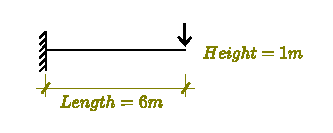
\includegraphics[width=7cm]{../Figure_files/4NodeANDES/cantilever_6.pdf}
  \caption{Problem description for cantilever beams}
  \label{fig Problem description for cantilever beams}
\end{figure}





\noindent \emph{\textbf{Numerical model:}}



The 27NodeBrick elements were shown in Figure (\ref{fig 8NodeBrick elements for cantilever beams}).

\begin{figure}[H]
  \centering
  \begin{subfigure}{0.5\textwidth}
    \centering
    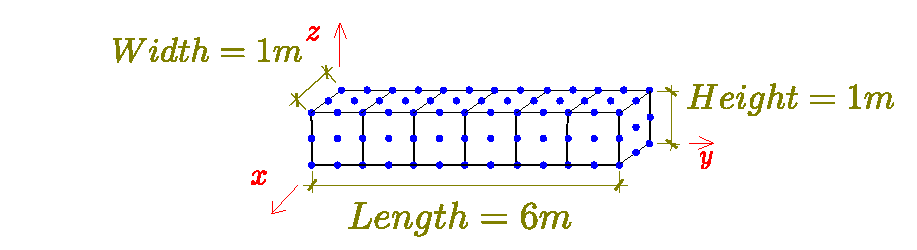
\includegraphics[width=9cm]{../Figure_files/27NodeBrick/beam_27brick_6div.pdf}
    % \caption{Six 8NodeBrick elements}
  \end{subfigure}
  \captionsetup{justification=centering,margin=3cm}
  \caption{27NodeBrick elements for cantilever beams}
  \label{fig 8NodeBrick elements for cantilever beams}
\end{figure}




\newpage
\section{4NodeANDES cantilever beams under the force perpendicular to plane}


\emph{\textbf{Problem description:}}


Length=6m, Width=1m, Height=1m, Force=100N, E=1E8Pa, $\nu=0.0$. The force direction was shown in Figure (\ref{fig Problem description for cantilever 4}). 

\begin{figure}[H]
  \centering
  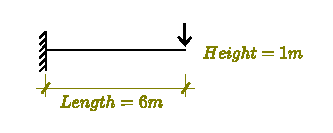
\includegraphics[width=7cm]{../Figure_files/4NodeANDES/cantilever_6.pdf}
  \caption{Problem description for cantilever beams}
  \label{fig Problem description for cantilever 4}
\end{figure}


\noindent \emph{\textbf{Numerical model:}}

\vskip 12pt


When the force direction is perpendicular to the plane, only the bending deformation is calculated in 4NodeANDES elements. 


The 4NodeANDES elements were shown in Figure (\ref{fig 4NodeANDES elements for cantilever beams under force perpendicular to plane}).

\begin{figure}[H]
  \centering
  \begin{subfigure}{0.5\textwidth}
    \centering
    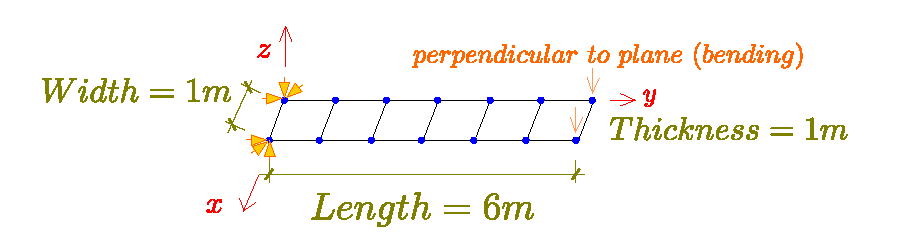
\includegraphics[width=9cm]{../Figure_files/4NodeANDES/beam_ANDES_xy_bending_6div.pdf}
    % \caption{Six 4NodeANDES elements}
  \end{subfigure}
  \captionsetup{justification=centering,margin=3cm}
  \caption{4NodeANDES elements for cantilever beams under force perpendicular to plane}
  \label{fig 4NodeANDES elements for cantilever beams under force perpendicular to plane}
\end{figure}









\newpage
\section{4NodeANDES cantilever beams under the inplane force}



\emph{\textbf{Problem description:}}

Length=6m, Width=1m, Height=1m, Force=100N, E=1E8Pa, $\nu=0.0$. The force direction was shown in Figure (\ref{fig Problem description for cantilever 4 2}). 

\begin{figure}[H]
  \centering
  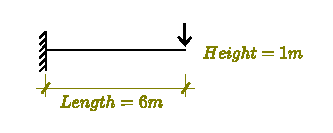
\includegraphics[width=7cm]{../Figure_files/4NodeANDES/cantilever_6.pdf}
  \caption{Problem description for cantilever beams}
  \label{fig Problem description for cantilever 4 2}
\end{figure}


\noindent \emph{\textbf{Numerical model:}}

When the force direction is inplane, both the bending and shear deformation are calculated in 4NodeANDES elements. 

The 4NodeANDES elements under inplane force were shown in Figure (\ref{fig 4NodeANDES elements for cantilever beams under inplane force}).

\begin{figure}[H]
  \centering
  \vskip 8pt
  \begin{subfigure}{0.5\textwidth}
    \centering
    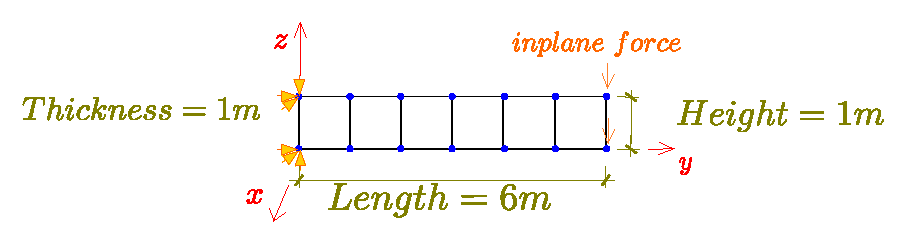
\includegraphics[width=9cm]{../Figure_files/4NodeANDES/beam_ANDES_yz_inPlane_6div.pdf}
    % \caption{Six 4NodeANDES elements}
  \end{subfigure}
  \captionsetup{justification=centering,margin=3cm}
  \caption{4NodeANDES elements for cantilever beams under inplane force}
  \label{fig 4NodeANDES elements for cantilever beams under inplane force}
\end{figure}




















\newpage
\section{4NodeANDES square plate with four edges clamped}



\emph{\textbf{Problem description:}}



Length=20m, Width=20m, Height=1m, Force=100N, E=1E8Pa, $\nu=0.3$. 

The four edges are \textbf{clamped}. 

The load is the uniform normal pressure on the whole plate. 


\begin{figure}[H]
  \centering
  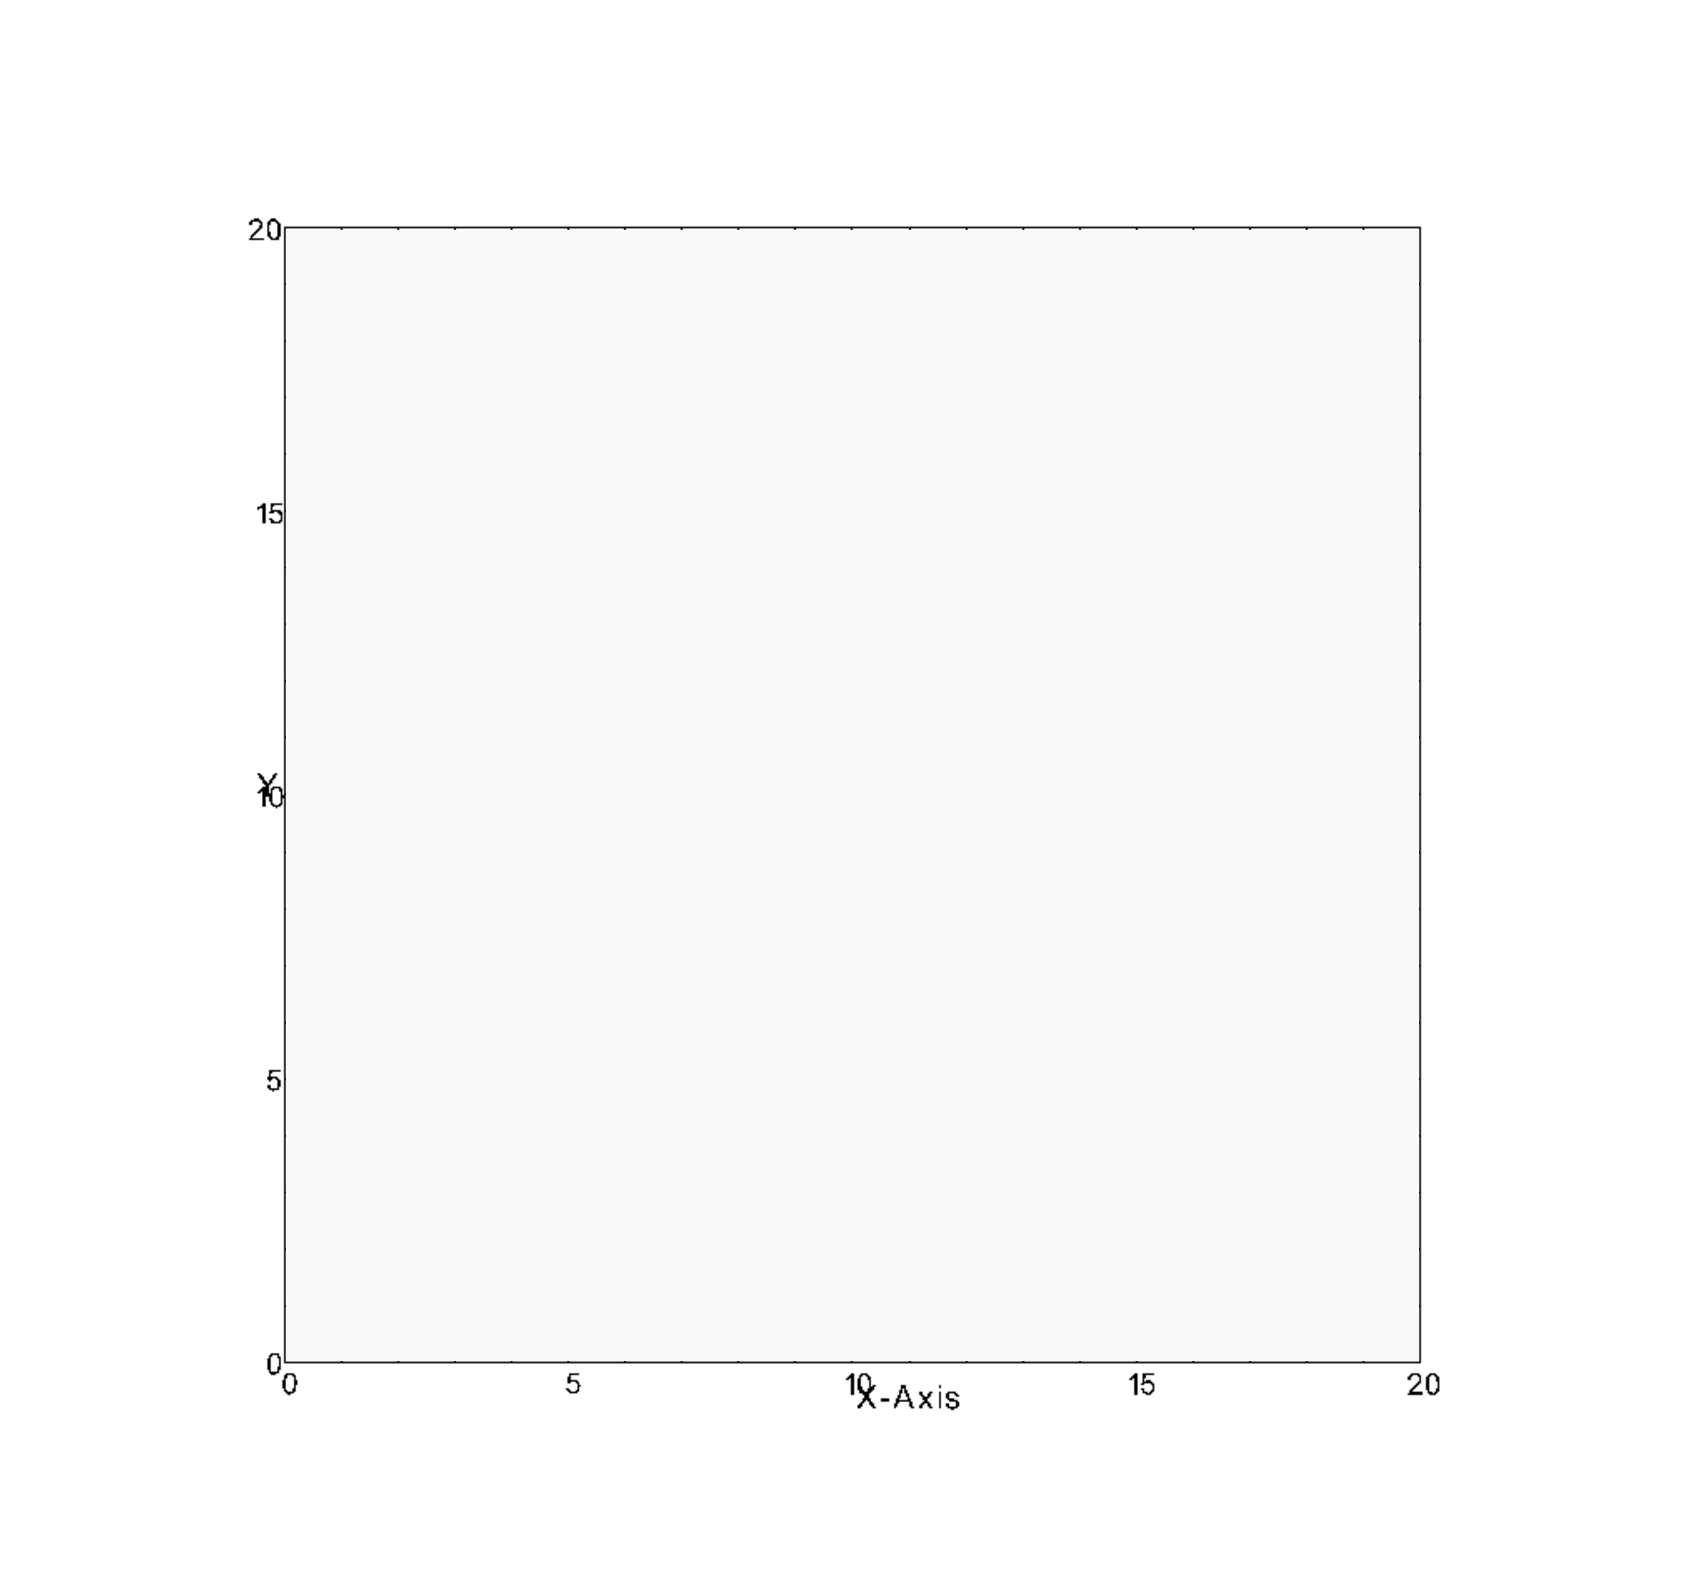
\includegraphics[width=11cm]{../Figure_files/4NodeANDES/square_plate_descrp.pdf}
  \caption{4NodeANDES edge clamped square plate with element side length 1m }
  \label{fig 4NodeANDES edges clamped square plate with element side length 1m }
\end{figure}


\newpage
\noindent \emph{\textbf{Numerical model:}}

The element side length is 1 meter. 


\begin{figure}[H]
  \centering
  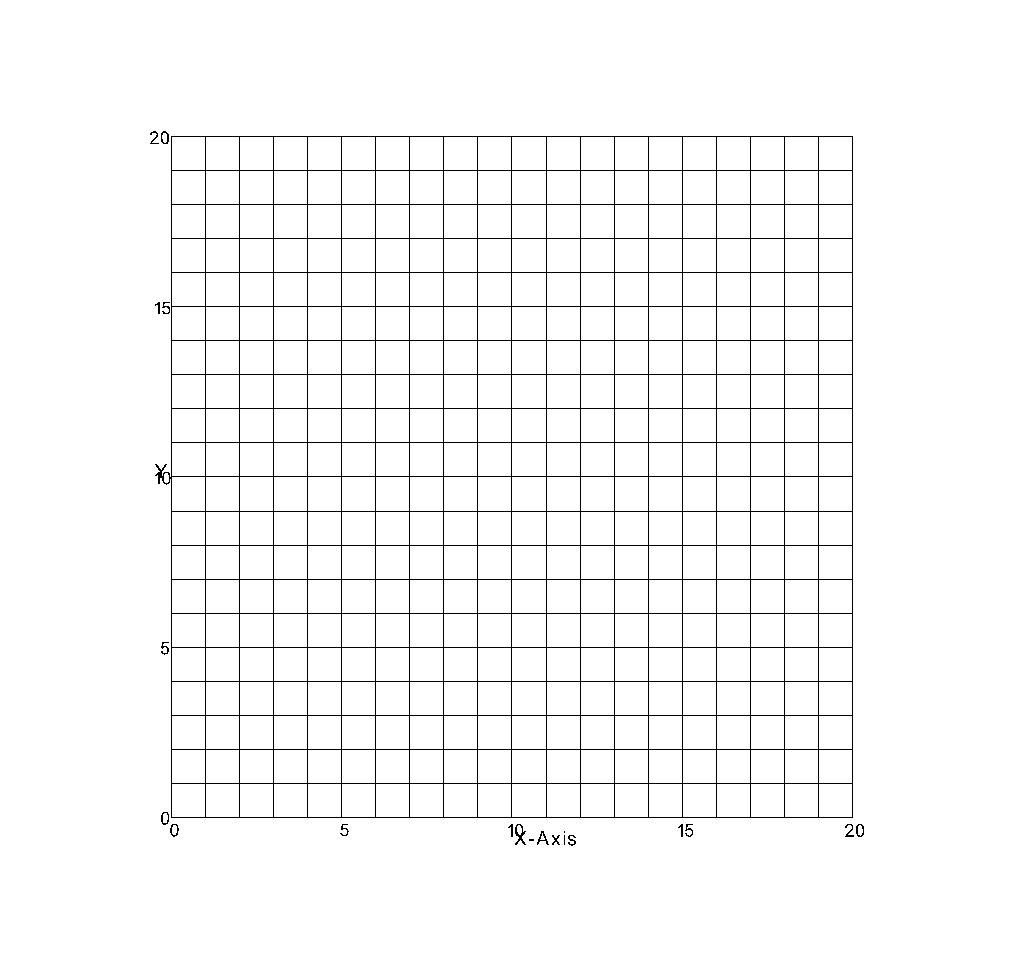
\includegraphics[width=11cm]{../Figure_files/4NodeANDES/square_plate4.png}
  \caption{4NodeANDES edge clamped square plate with element side length 1m }
  \label{fig 4NodeANDES edges clamped square plate with element side length 1m }
\end{figure}







\newpage
\section{The presentation example with beam\_elastic element}



\emph{\textbf{Problem description:}}

\begin{itemize}
  \item Structure size

    Structure length=6m, Width=6m, Height=6m, Force=100N 

  \item Element size

    Element length=6m, width=1m, height=1m, $\rho=0.0$, E=1E8Pa, $\nu=0.0$.
\end{itemize}





\begin{figure}[H]
  \centering
  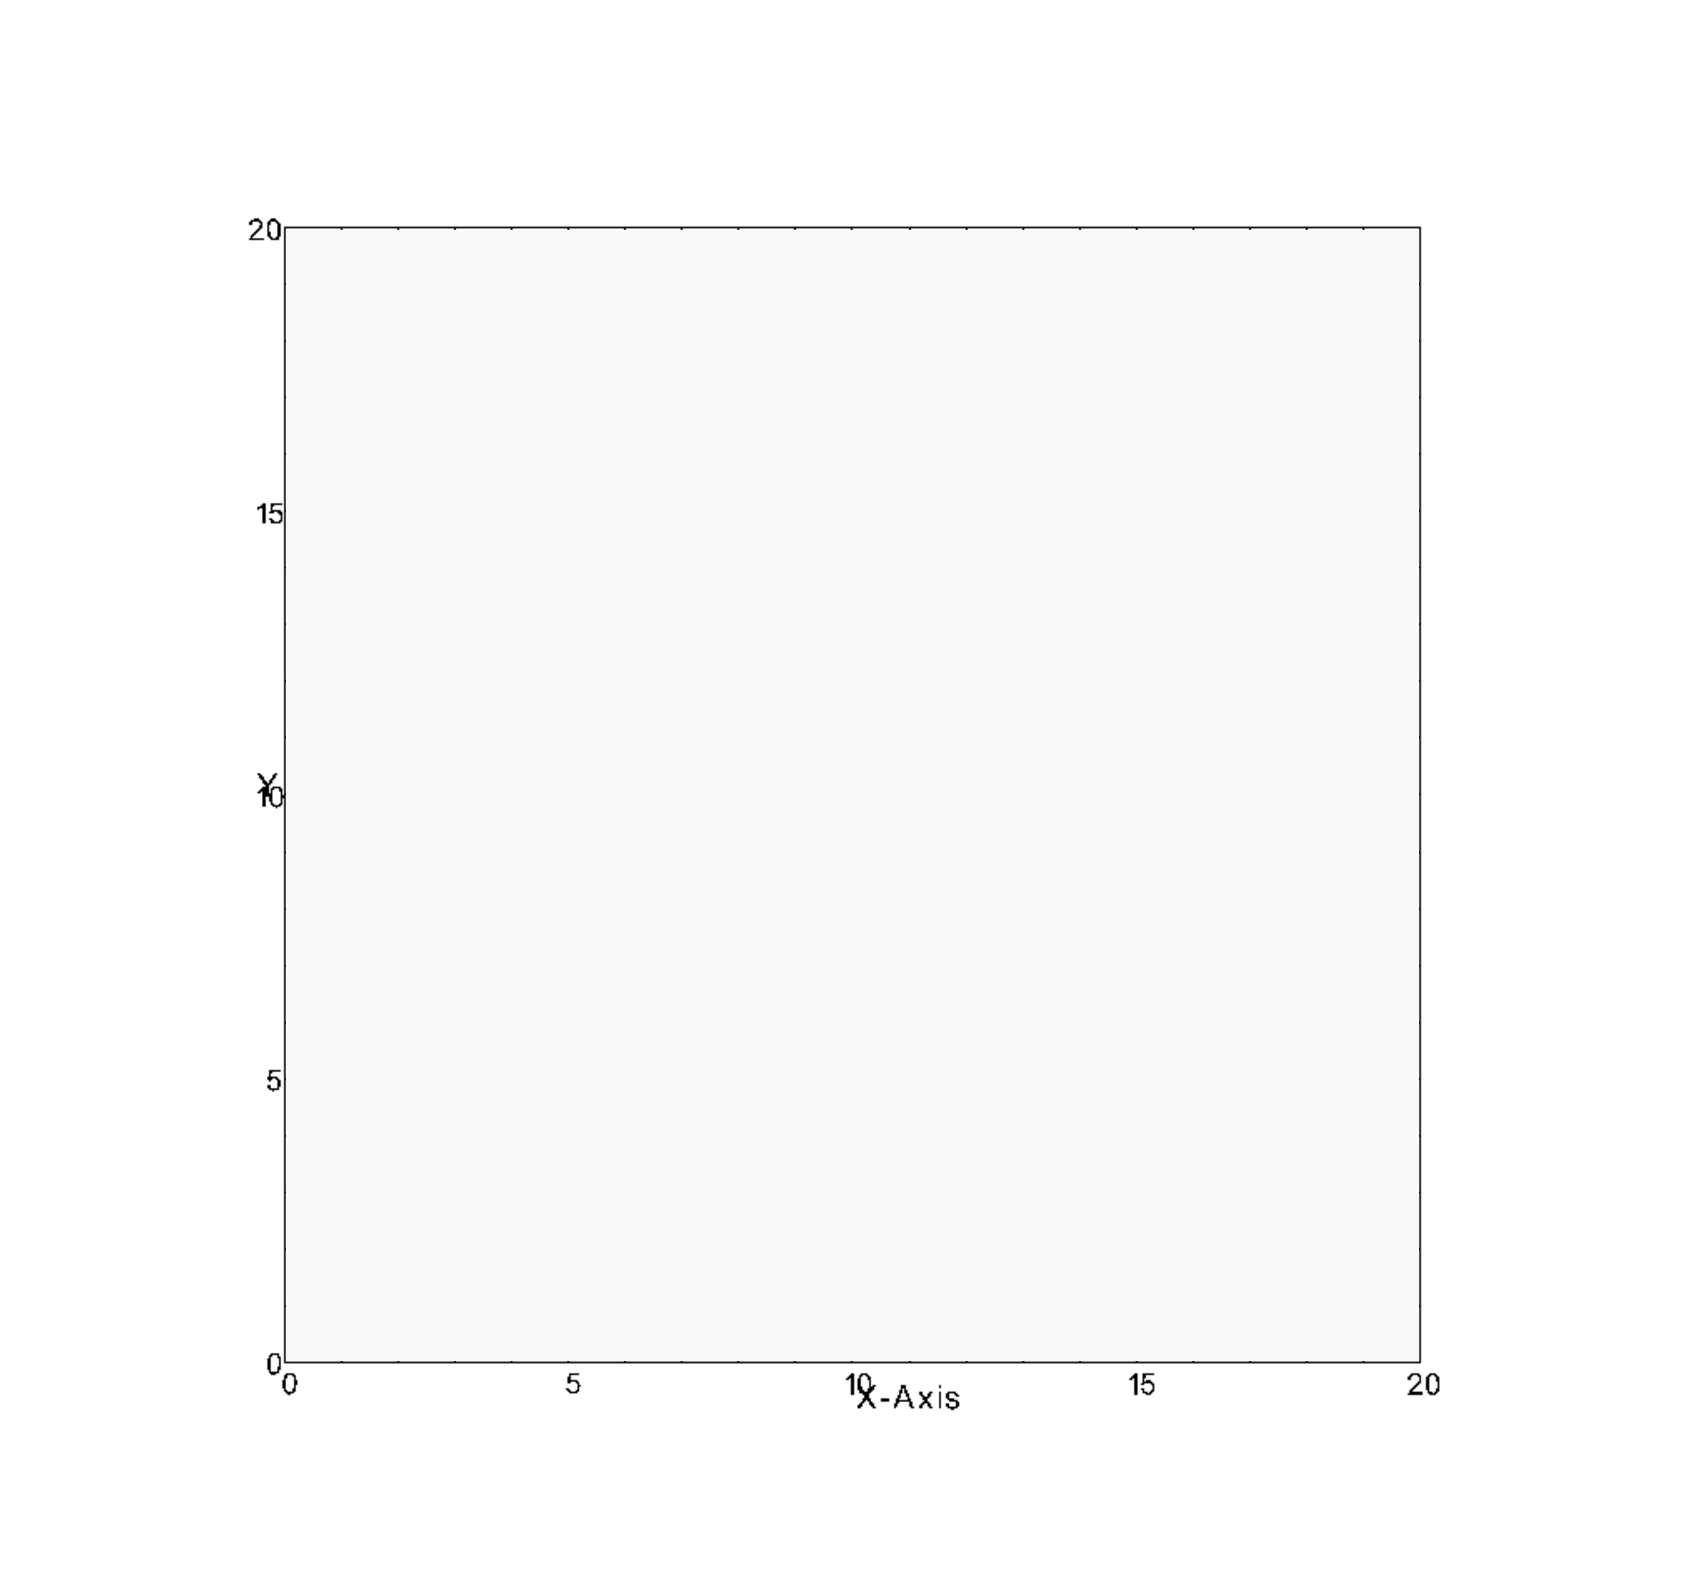
\includegraphics[width=11cm]{../Figure_files/4NodeANDES/square_plate_descrp.pdf}
  \caption{4NodeANDES edge clamped square plate with element side length 1m }
  \label{fig 4NodeANDES edges clamped square plate with element side length 1m }
\end{figure}


\newpage
\noindent \emph{\textbf{Numerical model:}}

The element side length is 1 meter. 


\begin{figure}[H]
  \centering
  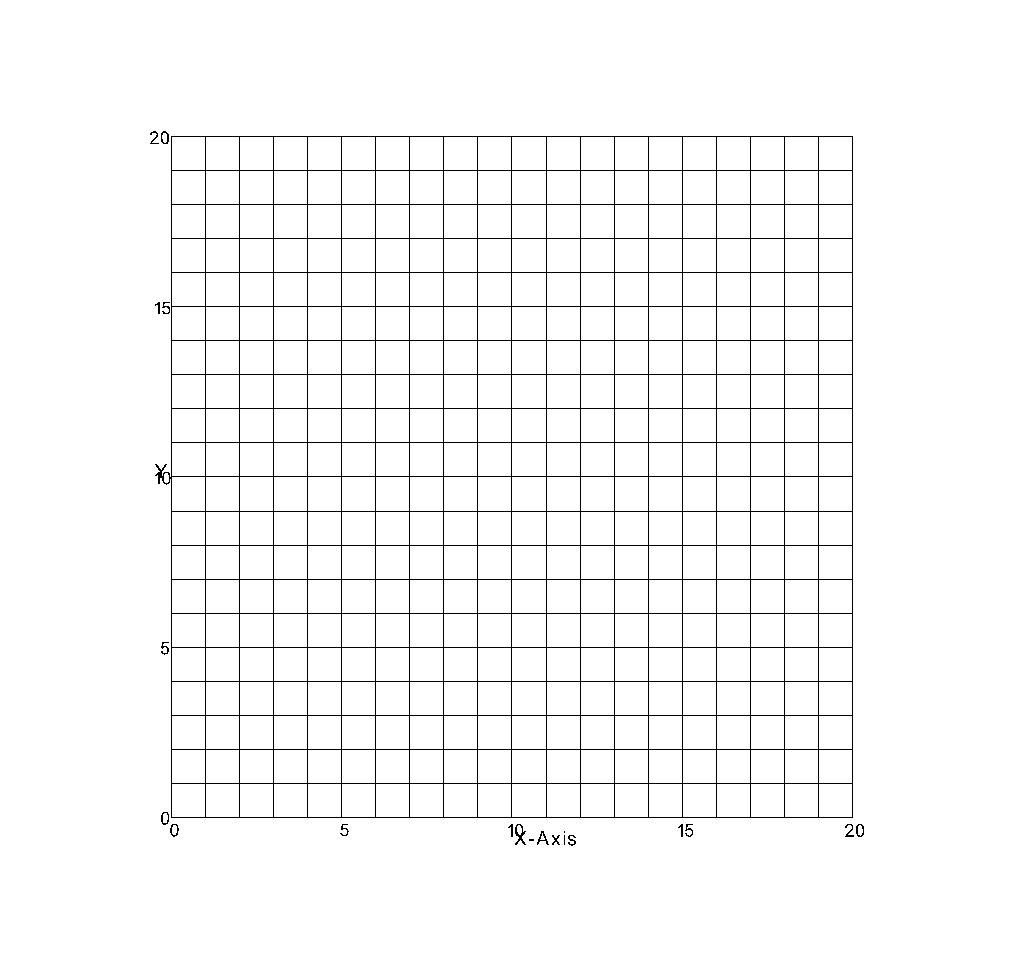
\includegraphics[width=11cm]{../Figure_files/4NodeANDES/square_plate4.png}
  \caption{4NodeANDES edge clamped square plate with element side length 1m }
  \label{fig 4NodeANDES edges clamped square plate with element side length 1m }
\end{figure}






%-------------------------------------------------------------------------------------------------------------%
%-------------------------------------------------------------------------------------------------------------%

\end{document}


        10        20        30        40        50        60        70        80
12345678901234567890123456789012345678901234567890123456789012345678901234567890
